%%%%%%%%%%%%%%%%%%%%%%%%%%%%%%%%%%%%%%%%%%%%%%%%%%%%%%%%%%%%%%%%%%%%%%
\documentclass[12pt,twoside]{article}
\usepackage{weiiszablon}
\usepackage{float}

\type{Projekt}
\subject{Sztuczna Inteligencja}
\title{Temat: Zrealizować sieć neuronową uczoną algorytmem wstecznej propagacji błędu z przyśpieszeniem metodą adaptacyjnego współczynnika uczenia (trainbpa)
uczącą się rozpoznawanie rodzaju wina}
\author{Szymon Kmieć}
\group{2EF-DI,	P2}

\begin{document}

% strona tytułowa
\maketitle

\blankpage

% spis treści
\tableofcontents

\clearpage
\blankpage


\section{Opis problemu}
Głównym celem projektu było zaprojektowanie oraz implementacja sieci neuronowej służącej do rozpoznawania gatunku wina. Do tego celu użyto własnej implementacji sieci neuronowej w języku Python 3.10.5 uczonej algorytmem wstecznej propagacji błędu. Jako metodę przyśpieszenia uczenia użyto adaptacyjnego współczynnika uczenia. W ramach projektu zbadano wpływ następujących parametrów na szybkość uczenia się sieci: 

%Głównym celem projektu było stworzenie algorytmu oraz nauczenie sieci neuronowej diagnozowania chorób na podstawie badań próbek tkanek z piersi. Została w tym celu stworzona sieć neuronowa uczona algorytmem wstecznej propagacji błędu. Jako metodę przyśpieszenia uczenia zastosowano adaptacyjny współczynnik uczenia. W ramach projektu zbadano wpływ parametrów na szybkość uczenia sieci:
\begin{itemize}
	\item S1 - liczba neuronów w pierwszej warstwie sieci
\item S2 - liczba neuronów w drugiej warstwie sieci
\item lr - współczynnik uczenia sieci
\item er - współczynnik maksymalnego dopuszczalnego przyrostu błędu, oznaczany również jako MAX\_PERF\_INC
\item lr\textsubscript{dec} - modyfikator współczynnika uczenia w przypadku przekroczeniu maksymalnego dopuszczalnego przyrostu błędu
\item lr\textsubscript{inc} - modyfikator współczynnika uczenia w przypadku spadku błędu
\end{itemize}

Opis problemu oraz wykorzystane w projekcie dane zostały przedstawione na stronie \cite{dane}

\clearpage

\section{Specyfikacja danych}
Dane pobrane z wspomnianej powyżej strony zawierały 178 wierszy danych, z których to każdy posiadał 14 atrybutów (w tym atrybut klasowy). Dane
są wynikiem analizy chemicznej win uprawianych w tym samym regionie Włoch,
ale pochodzących z trzech różnych odmian. Badany zestaw danych nie zawiera
niekompletnych rekordów, oraz wartości niepoprawnych. W zbiorze danych pierwszy
atrybut określa rodzaj wina - opisany liczbą całkowitą {1, 2, 3}, natomiast pozostałe
13 atrybutów to
\begin{itemize}
\item (Alcohol) - Procentowa zawartość alkoholu (wartość ciągła)
\item (Malic acid) - Procentowa zawartość kwasu jabłkowego (wartość ciągła)
\item (Ash) - Zawartość popiołu (wartość ciągła)
\item (Alkalinity of ash) - Zasadowość popiołu (wartość ciągła)
\item (Mg) - Zawartość magnezu (wartość ciągła)
\item (Total phenols) - Zawartość fenoli (wartość ciągła)
\item (Flavonoids) - Flawonoidy (wartość ciągła)
\item (Non Flavonoid phenols) - Fenole nieflawonoidowe (wartość ciągła)
\item (Proanthocyanins) - Proantocyjanidyny (wartość ciągła)
\item (Colour intensity) - Intensywność barwy (wartość ciągła)
\item (Hue) - Odcień (wartość ciągła)
\item (OD280/0D315) (wartość ciągła)
\item (Proline) - Prolina (wartość dyskretna)
\end{itemize}
\clearpage

\subsection{Normalizacja danych}
W celu usprawnienia procesu uczenia dane wejściowe zostaly poddane normalizacji metodą \textit{min - max} określoną wzorem \cite{norm}:
\begin{equation}
f(x) = \frac{x - \min{(x)}}{\max{(x)} - \min{(x)}}
\end{equation}


Dzięki takiej normalizacji, możliwe jest dynamiczne normalizowanie danych wejściowych do zadanego zakresu. W przypadku tego projektu został zastosowany przedział normalizacyjny $ [0, 1]$.\\

\begin{lstlisting}[language=Python,caption=Algorytm normalizacji,label={Kod1}]
    for column in norm_data.columns:
        if column !=0:
            norm_data[column] = (norm_data[column] - norm_data[column].min()) / (norm_data[column].max() - norm_data[column].min())

\end{lstlisting}

Numery klas, stanowiące dane wyjściowe, zostały natomiast przekształcone przy pomocy kodowania 1 z N do postaci trójelementowego wektora, zawierającego wartość 1 na pozycji odpowiadającej danej klasie oraz wartości 0 na pozostałych pozycjach.



\clearpage
\section{Zagadnienia teoretyczne}
\subsection{Model sztucznego neuronu}
Podstawowym elementem z którego zbudowane są sieci neuronowe jest pojedynczy neuron. Neuron jest jednostką która przetwarza informacje wejściowe, oraz zwraca wynik przetwarzania w postaci wartości wyjściowej. 


Początkowo neuron miał co najmniej jedno wejście binarne i tylko jedno binarne wyjście. Wyjście było aktywowane, gdy osiągnięta została określona liczba wejść. W 1957 roku uczony Frank Rosenblatt zmodyfikował prosty sztuczny neuron binarny, tworząc w ten sposób perceptron, czyli jedną z najprostszych sieci neuronowych. Posiada on następującą charakterystykę \cite{mamczur}:
\begin{itemize}
\item Na wejściu i wyjściu zamiast wartości binarnych mogą być dowolne liczby
\item Połączenia węzłów mają nadaną wagę
\item Wartość wyjściowa w węźle składa się z dwóch części: sumy wartości z warstw poprzednich pomnożonej przez wagi oraz nałożonej na tą sumę funkcji aktywacji.
\end{itemize}

Na rysunku \ref{neuron} sygnał przechodzi z lewej do prawej.

\begin{figure}[ht]
\label{neuron}
\centering
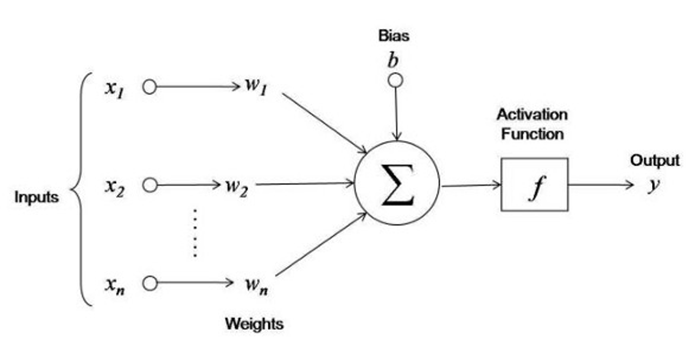
\includegraphics[width=14cm]{neuron.png}
\caption{Model neuronu}
\end{figure}

Ważona suma wejść wraz z przesunięciem nazywana jest łącznym pobudzeniem neuronu i określana wzorem:
\begin{equation}\label{pobudzenie}
z = \sum_{i=1}^{n}(x_i \cdot w_i) + b 
\end{equation}

Ogólny wzór na wartość wyjścia neuronu przedstawiono równaniem \ref{wyj-neu}

\begin{equation}\label{wyj-neu}
y = f \left(  \sum_{i=1}^{n}(x_i \cdot w_i) + b \right) = f(z)
\end{equation}
gdzie:
\begin{itemize}
\item $y$ - wyjście neuronu
\item $f$ - funkcja aktywacji
\item $n$ - ilość wejść
\item $x$ - wektor wejciowy
\item $w$ - wektor wag
\item $b$  - bias
\end{itemize}
Ze względu na funkcję aktywacji wyróżnia się różne typy neuronów. Najczęściej stosowanymi funkcjami aktywacji neuronu są funkcje liniowe (\ref{lin}) oraz sigmoidalne (\ref{siguni} oraz \ref{sigbi}).


Funkcja liniowa ma postać:
\begin{equation}\label{lin}
f(x) = a \cdot x + b
\end{equation}

Funkcja sigmoidalna unipolarna:
\begin{equation}\label{siguni}
f(x) = \frac{1}{1 + e^{-\beta x}}
\end{equation}

Funkcja sigmoidalna bipolarna:
\begin{equation}\label{sigbi}
f(x) = \frac{2}{1 + e^{-\beta x}} -1
\end{equation}

gdzie parametr $\beta$ określony jest z reguły w przedziale $[0, 1]$.
\clearpage

\subsection{Sieć jednokierunkowa wielowarstwowa}

Sztuczną sieć neuronowa uzyskuje się łącząc ze sobą warstwy neuronów. Przykładowy model sieci wielowarstwowej pokazano na rysunku \ref{wielo}.

\begin{figure}[h]
\label{wielo}
\centering
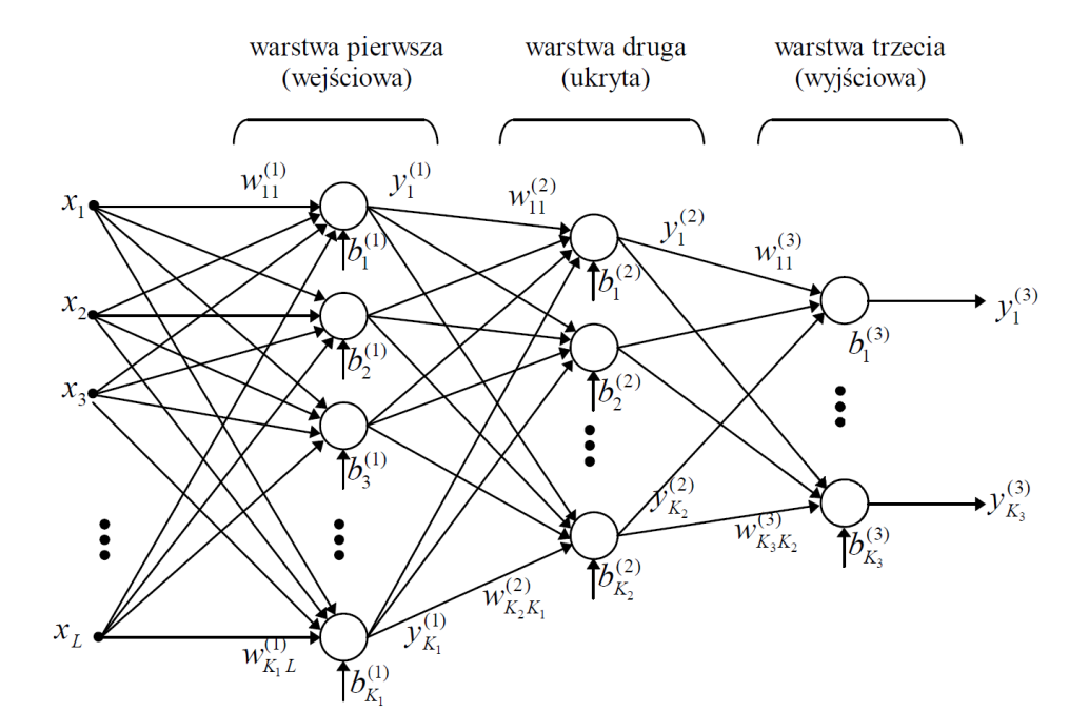
\includegraphics[width=14cm]{wielowarstwowa.png}
\caption{Sieć jednokierunkowa wielowarstwowa	[Źródło: \cite{zajdel1}]}
\end{figure}

Sieć taka ma zwykle strukturę obejmującą: 
\begin{itemize}
\item warstwę wejściową
\item co najmniej jedną warstwę ukrytą (złożoną z neuronów sigmoidalnych)
\item warstwę wyjściową (złożoną z neuronów sigmoidalnych lub liniowych)
\end{itemize}

Każda warstwa posiada:
\begin{itemize}
\item Macierz wag neuronów - $\textbf{w}$
\item Wektor przesunięć - $\textbf{b}$
\item Wektor sygnałów wyjściowych - $\textbf{y}$
\end{itemize}

Działanie poszczególnych warstw sieci opisane jest wzorami:
\begin{equation}\label{warstwy}
\begin{aligned}
y^{(1)} &= f^{(1)}(w^{(1)}x + b^{(1)})\\
y^{(2)} &= f^{(2)}(w^{(2)}y^{(1)} + b^{(2)})\\
y^{(3)} &= f^{(3)}(w^{(3)}y^{(2)} + b^{(3)})
\end{aligned}
\end{equation}

Zatem działanie całej trójwarstwowej sieci można zapisać jako:
\begin{equation}
y^{(3)} = f^{(3)}\left( w^{(3)} f^{(2)} \left( w^{(2)}f^{(1)} \left( w^{(1)}x + b^{(1)}\right) + b^{(2)} \right) + b^{(3)} \right)
\end{equation}
\\


\subsection{Uczenie sieci algorytmem wstecznej propagacji błędu}

Algorytm wstecznej propagacji błędu dominuje wśród metod uczenia sieci jednokierunkowych. Opiera się on na koncepcji poprawiania na każdym kroku procesu uczenia wartości korekty wag na podstawie oceny błędu popełnionego przez każdy neuron podczas uczenia sieci \cite{leksykon}. 

Do zastosowania algorytmu wstecznej propagacji błędu, wymagane jest, aby funkcje aktywacji neuronów były różniczkowalne, co pozwala na wyznaczenie pochodnej błędu po danych wyjściowych. Dla każdej pary $(x, \hat{y})$ sieć popełnia błąd, który można zdefiniować następująco:

\begin{equation}
e = y - \hat{y}
\end{equation}

Celem uczenia sieci jest zminimalizowanie sumarycznego błędu kwadratowego, wyrażonego jako suma kwadratów błędów dla K neuronów w warstwie wyjściowej.
\begin{equation}\label{sredniokwad}
E = \frac{1}{2} \sum_{j=1}^{K} e_{j}^2
\end{equation}

W przypadku sieci z rysunku \ref{wielo} funkcja \ref{sredniokwad} po uwzględnieniu zależności \ref{warstwy} przyjmie postać:

\begin{equation}
\begin{aligned}
E =& \frac{1}{2} \sum_{i_{3}=1}^{K_{3}} e_{i_{3}}^2 = \frac{1}{2} \sum_{i_{3}=1}^{K_{3}}\left( y_{i_{3}}^{(3)} - \hat{y}_{i_{3}} \right)^2 =\\
 =& \frac{1}{2} \sum_{i_{3}=1}^{K_{3}} \left( f^{(3)}\left( \sum_{i_{2}=1}^{K_{2}} w_{i_{3}j_{2}}^{(3)}y_{i_{2}} + b_{i_{3}}^{(3)} \right) - \hat{y}_{i_{3}} \right)^2 =\\
=& \frac{1}{2} \sum_{i_{3}=1}^{K_{3}} \left( f^{(3)}\left( \sum_{i_{2}=1}^{K_{2}} w_{i_{3}j_{2}}^{(3)} f^{(2)}\left( \sum_{i_{1}=1}^{K_{1}} w_{i_{2}j_{1}}^{(2)} y_{i_{1}} + b_{i_{2}}^{(2)} \right) + b_{i_{3}}^{(3)} \right) - \hat{y}_{i_{3}} \right)^2 =\\
=& \frac{1}{2} \sum_{i_{3}=1}^{K_{3}} \left( f^{(3)}\left( \sum_{i_{2}=1}^{K_{2}} w_{i_{3}j_{2}}^{(3)} f^{(2)}\left( \sum_{i_{1}=1}^{K_{1}} w_{i_{2}j_{1}}^{(2)} f^{(1)}\left( \sum_{j=1}^{L} w_{i_{1}j}^{(1)} x_{j} + b_{i_{1}}^{(1)} \right) + b_{i_{2}}^{(2)} \right) + b_{i_{3}}^{(3)} \right) - \hat{y}_{i_{3}} \right)^2 
\end{aligned}
\end{equation}\\

Zminimalizowanie błędu \ref{sredniokwad} osiąga się poprzez zmianę biasów neuronów oraz wag ich połączeń. Kolejna wartość wagi połączenia jest wyznaczana na podstawie pochodnej cząstkowej błędu po wartości tejże wagi w obecnym cyklu nauczania. W podobny sposób wyznaczana jest również nowa wartość biasu dla każdego z neuronów. Otrzymaną pochodną mnoży się przez współczynnik uczenia $\eta$, który również może zmieniać się podczas procesu uczenia sieci. Wagę dla $k+1$ kroku otrzymać można w następujący sposób:\\
\begin{equation}
w_{ij}(k+1) = w_{ij}(k) - \eta \frac{\partial E}{\partial w_{ij}(k)}
\end{equation}\\

Zatem zmiany wag obliczane są ze wzoru:\\
\begin{equation}
\Delta w_{ij} = - \eta \frac{\partial E}{\partial w_{ij}}
\end{equation}\\

Obliczanie wag neuronów rozpoczyna się od warstwy wyjściowej:\\
\begin{equation}
\frac{\partial E}{\partial w_{i_{3}i_{2}}^{(3)}} = \frac{\partial E}{\partial f^{(3)}} \frac{\partial f^{(3)}\left( z_{i_{3}}^{(3)} \right)}{\partial z_{i_{3}}^{(3)}} \frac{\partial z_{i_{3}}^{(3)}}{\partial w_{i_{3}i_{2}}^{(3)}} = \left( y_{i_{3}} - \hat{y}_{i_{3}} \right) \frac{\partial f^{(3)}\left( z_{i_{3}}^{(3)} \right)}{\partial z_{i_{3}}^{(3)}} y_{i_{2}}^{(2)}
\end{equation}\\
\newpage
Podobnie można obliczyć elementy gradientu względem wag warstwy ukrytej\\
\begin{equation}
\begin{aligned}
&\frac{\partial E}{\partial w_{i_{2}i_{1}}^{(2)}} = \frac{\partial E}{\partial f^{(3)}} \frac{\partial f^{(3)}\left( z_{i_{3}}^{(3)} \right)}{\partial z_{i_{3}}^{(3)}} \frac{\partial z_{i_{3}}^{(3)}}{\partial f^{(2)}} \frac{\partial f^{(2)}\left( z_{i_{2}}^{(2)} \right)}{\partial z_{i_{2}}^{(2)}} \frac{\partial z_{i_{2}}^{(2)}}{\partial w_{i_{2}i_{1}}^{(2)}}  =\\
&= \sum_{i_{3}=1}^{K_3}\left( y_{i_{3}} - \hat{y}_{i_{3}} \right) \frac{\partial f^{(3)}\left( z_{i_{3}}^{(3)} \right)}{\partial z_{i_{3}}^{(3)}} w_{i_{3}i_{2}}^{(3)} \frac{\partial f^{(2)}\left( z_{i_{2}}^{(2)} \right)}{\partial z_{i_{2}}^{(2)}} y_{i_{1}}^{(1)}
\end{aligned}
\end{equation}\\

Oraz dla warstwy wejściowej\\
\begin{equation}
\begin{aligned}
&\frac{\partial E}{\partial w_{i_{1}j}^{(1)}} = \frac{\partial E}{\partial f^{(3)}} \frac{\partial f^{(3)}\left( z_{i_{3}}^{(3)} \right)}{\partial z_{i_{3}}^{(3)}} \frac{\partial z_{i_{3}}^{(3)}}{\partial f^{(2)}} \frac{\partial f^{(2)}\left( z_{i_{2}}^{(2)} \right)}{\partial z_{i_{2}}^{(2)}} \frac{\partial z_{i_{2}}^{(2)}}{\partial f^{(1)}}  \frac{\partial f^{(1)}\left( z_{i_{1}}^{(1)} \right)}{\partial z_{i_{1}}^{(1)}} \frac{\partial z_{i_{1}}^{(1)}}{\partial w_{i_{1}j}^{(1)}}  =\\
&= \sum_{i_{3}=1}^{K_3}\left( y_{i_{3}} - \hat{y}_{i_{3}} \right) \frac{\partial f^{(3)}\left( z_{i_{3}}^{(3)} \right)}{\partial z_{i_{3}}^{(3)}} \sum_{i_{2}=1}^{K_2} w_{i_{3}i_{2}}^{(3)} \frac{\partial f^{(2)}\left( z_{i_{2}}^{(2)} \right)}{\partial z_{i_{2}}^{(2)}} w_{i_{2}i_{1}}^{(2)} \frac{\partial f^{(1)}\left( z_{i_{1}}^{(1)} \right)}{\partial z_{i_{1}}^{(1)}} x_j
\end{aligned}
\end{equation}
\\
\subsection{Adaptacyjny współczynik uczenia}

Algorytm wstecznej propagacji błędu jest dość czasochłonny. W celu przyśpieszenia procesu uczenia sieci korzysta się z metod pozwalających na jego przyśpieszenie. Jedną z nich jest metoda adaptacyjnej korekty współczynnika uczenia. Decyzję o zmianie podejmuje się na podstawie porównania błędu kwadratowego z jego wartością uzyskaną w poprzednim cyklu nauczania. Kolejną wartość $\eta$ otrzymuje się na podstawie następującej zależności:

\begin{equation}
\eta (t + 1) =
\left\{\begin{aligned}
\eta (t)  \xi_d  & \qquad gdy\ SSE(t) > er \cdot SSE(t - 1)\\
\eta (t)  \xi_i  & \qquad gdy\ SSE(t) < SSE(t - 1)\\
\eta (t)   & \qquad gdy\ SSE(t - 1) \leq SSE(t) \leq er \cdot SSE(t - 1)
\end{aligned}\right.
\end{equation}

gdzie:
\begin{itemize}
\item $er$ - dopuszczalna krotność przyrostu błędu
\item $\xi_d$ - współczynnik zmniejszania wartości współczynnika uczenia
\item $\xi_i$ - współczynnik zwiększania wartości współczynnika uczenia
\end{itemize}
\clearpage

\section{Algorytm}

Na potrzeby realizacji projektu zaimplementowano w języku Python algorytm pozwalający na uczenie dowolnej sieci neuronowej algorytmem wstecznej propagacji błędu, wraz z przyspieszeniem metodą adaptacyjnego współczynnika uczenia. 

Python jest z natury językiem wolnym. Dzieje się tak, ponieważ należy do grupy języków interpretowanych. Z racji tego, implementacja sieci w samym Pythonie byłaby nieefektywna. W związku z tym do obliczeń wykorzystano moduł \textit{numpy}. Biblioteka ta została napisana i skompilowana w języku C, dlatego wykonywanie obliczeń będzie znacznie przyspieszone. Do kroswalidacji użyto modułu \textit{sklearn}.

Algorytm oferuje możliwość wyboru techniki aktualizacji wag:
\begin{itemize}
\item Wsadowa -  parametry neuronów aktualizowane są dopiero po wczytaniu do sieci całego zestawu danych uczących
\item Mini-batch -  Zbiór danych podzielony jest na podzbiory, aktualizacja parametrów sieci następuje po zaprezentowaniu całego podzbioru

\end{itemize}

\begin{lstlisting}[language=Python,caption=Algorytm uczenia sieci,label={Kod2}]
import random
import numpy as np


class Network(object):
    """konstruktor obiektu sieci - przyjmuje jako parametr liste 
    zawierajaca liczbe wejsc, liczbe neuronow w 
    warstwach S1, S2, oraz liczbe neuronow na wyjsciu"""
    def __init__(self, sizes, err=1.04):
        #do ilosci warstw sieci przypisz dlugosc wektora "sizes"
        self.num_layers = len(sizes)
        #przypisanie wektora do zmiennej w obiekcie
        self.sizes = sizes
        #ustawia parametry generatora pseudolosowego
        #aby kolejnym sieciom byly przypisywane takie same wagi 
        #i biasy
        np.random.seed(1)
        """inicjalizacja biasow i wag przy pomocy rozkladu 
        gaussa N(0,1) dla wszystkich warstw poza zerowa 
        (warstwa wejsciowa to nie neurony)"""
        self.biases = [np.random.randn(y, 1) for y in sizes[1:]]
        self.weights = [np.random.randn(y, x)
                        for x, y in zip(sizes[:-1], sizes[1:])]
        #maksymalny przyrost bledu
        self.max_perf_inc = err

    def feedforward(self, a):
        #zwraca wynik sieci neuronowej dla zestawu danych "a"
        for b, w in zip(self.biases, self.weights):
            a = sigmoid(np.dot(w, a)+b)
        return a
    
    #liczenie bledu sredniokwadratowego
    def sse(self,_test_data):
        error=[pow(np.linalg.norm(self.feedforward(x)-y),2) for (x,y) in _test_data]
        return 0.5*sum(error)    

    
    def SGD(self, training_data, epochs, mini_batch_size, eta,
            test_data,error_goal,inc,dec):
        """Funkcja odpowiedzialna za proces uczenia.
        Jako parametry przyjmuje: liste krotek (x, y)
        gdzie x - wektor danych uczacych, 
        y - oczekiwane wyjscie sieci;
        maksymalna liczbe epok; rozmiar podzbioru danych;
        poczatkowy wspolczynnik uczenia; liste krotek (x, y)
        zawierajacych dane testowe; docelowy koszt;
        wspolczynnik przyrostu i spadku wspolczynnika uczenia"""
        #przypisanie do zmiennej ilosci testow
        n_test = len(test_data)
        n = len(training_data)
        #petla dla kazdej epoki
        for j in range(epochs):
            #przelosowanie zbioru uczacego
            random.shuffle(training_data)
            #generowanie podzbiorow
            mini_batches = [training_data[k:k+mini_batch_size]
                    for k in range(0, n, mini_batch_size)]
            #obliczanie bledu dla starych parametrow
            old_error=self.sse(test_data)
            #kopia zapasowa wektorow z biasami i wagami
            backup_weights = self.weights.copy()
            backup_biases = self.biases.copy()
            #aktualizowanie kazdego z podzbiorow
            for mini_batch in mini_batches:
                self.update_mini_batch(mini_batch, eta)
            #obliczenie bledu dla nowych wartosci bias i wag
            new_error=self.sse(test_data)
            #jezeli nowy blad < pozadany koszt
            if new_error < error_goal:
                #obliczanie sprawnosci sieci
                #evaluate - liczba poprawnych dopasowan
                test=self.evaluate(test_data)
                #zamiana na wartosc procentowa
                test2=test/n_test*100
                print("Epoch {0}: , {1:.2f}%".format(j+1,  test2))             
                return [j+1, test2]
            #jezeli nowy blad < starego
            elif new_error < old_error:
                #zwiekszenie wspolczynnika uczenia 
                eta *= inc
            #jezeli nowy blad > stary * max przyrost bledu
            elif new_error > old_error * self.max_perf_inc:
                #przywrocenie starych biasow i wag
                self.weights = backup_weights
                self.biases = backup_biases
                #zmniejszenie wspolczynnika uczenia
                eta *= dec
            #jezeli uplynela max liczba epok 
            if j==epochs-1:
                test=self.evaluate(test_data)
                test2=test/n_test*100
                print("Epoch {0}: , {1:.2f}%".format(j+1,  test2))
                return [j+1, test2]

    def update_mini_batch(self, mini_batch, eta):
        #Funkcja aktualizujaca wagi i biasy poprzez 
        #zastosowanie metody gradientowej i wstecznej 
        #propagacji dla danego podzioru. Jako parametry 
        #przyjmuje: liste krotek (x, y) oraz wspolczynik uczenia
        #generowanie macierzy zerowej dla gradientu biasow i wag
        nabla_b = [np.zeros(b.shape) for b in self.biases]
        nabla_w = [np.zeros(w.shape) for w in self.weights]
        
        for x, y in mini_batch:
            #dla kazdej pary (x, y) oblicz przyrost gradientu
            delta_nabla_b, delta_nabla_w = self.backprop(x, y)
            #oblicz nowy gradient
            nabla_b = [nb+dnb for nb, dnb in zip(nabla_b, delta_nabla_b)]
            nabla_w = [nw+dnw for nw, dnw in zip(nabla_w, delta_nabla_w)]
        #obliczanie nowych wag i biasow
        self.weights = [w-(eta/2)*nw
                        for w, nw in zip(self.weights, nabla_w)]
        self.biases = [b-(eta/2)*nb
                       for b, nb in zip(self.biases, nabla_b)]

    def backprop(self, x, y):
        """Zwraca krotke (nabla_b, nabla_w) rezprezentujaca 
        gradient funkcji kosztu"""
        nabla_b = [np.zeros(b.shape) for b in self.biases]
        nabla_w = [np.zeros(w.shape) for w in self.weights]
        # feedforward
        #
        activation = x
        #lista zawierajaca aktywacje wszystkich neuronow, 
        #warstwa po warstwie
        activations = [x]
        # lista pobudzen, warstwa po warstwie
        zs = []
        #obliczanie aktywacji i pobudzen
        for b, w in zip(self.biases, self.weights):
            z = np.dot(w, activation)+b
            zs.append(z)
            activation = sigmoid(z)
            activations.append(activation)
        #obliczanie przyrostu gradientu dla warstwy wyjsciowej
        delta = self.cost_derivative(activations[-1], y) * \
            sigmoid_prime(zs[-1])
        nabla_b[-1] = delta
        nabla_w[-1] = np.dot(delta, activations[-2].transpose())
        #obliczanie przyrostu gradientu dla warstwy ukrytej i 
        #wejsciowej
        for l in range(2, self.num_layers):
            z = zs[-l]
            sp = sigmoid_prime(z)
            delta = np.dot(self.weights[-l+1].transpose(), delta) * sp
            nabla_b[-l] = delta
            nabla_w[-l] = np.dot(delta, activations[-l-1].transpose())
        return (nabla_b, nabla_w)

    def evaluate(self, test_data):
        """Zwraca liczbe poprawnie dopasowanych rekordow 
        treningowych. Jako argument przyjmuje liste krotek (x,y) 
        z danymi testowymi"""
        """tworzy liste krotek gdzie x - indeks neuronu ktory 
        posiada najwieksza wartosc, y - oczekiwana klasa"""
        test_results = [(np.argmax(self.feedforward(x)), np.argmax(y))
                        for (x, y) in test_data]
        #suma poprawnych dopasowan
        return sum(int(x == y) for (x, y) in test_results)

    def cost_derivative(self, output_activations, y):
        #Funkcja zwracajaca wektor 
        #(atywacja neuronow - oczekiwane wyniki)
        return (output_activations-y)

def sigmoid(z):
    """Funkcja sigmoidalna"""
    return 1.0/(1.0+np.exp(-z))

def sigmoid_prime(z):
    """Pochodna z funkcji sigmoidalnej"""
    return sigmoid(z)*(1-sigmoid(z))

\end{lstlisting}
\clearpage

\section{Eksperymenty}


\subsection{Eksperyment 1 - badanie wpływu S1 i S2 na szybkość uczenia sieci}

Celem eksperymentu było znalezienie takiej kombinacji parametrów S1 oraz S2, dla której sieć osiągnie najlepszą poprawność klasyfikacji. Listing \ref{eks1} przedstawia kod odpowiedzialny za tenże eksperyment. Każda instancja sieci neuronowej została zainicjalizowana takimi samymi wagami i biasami. Do przeprowadzenia eksperymentu przyjęto następujące wartości domyślne:

\begin{table}[H]
\begin{center}
\begin{tabular}{|c|c|}
\hline
S1 (neurony warstwy I) & $[1, 20]$\\
\hline
S2 (neurony warstwy II) & $[1, 20]$\\
\hline
Learning rate & 0.1\\
\hline
Learning rate accelerate & 1.05\\
\hline
Learning rate decelerate & 0.7\\
\hline
Error ratio & 1.04\\
\hline
Stosunek wielkości zbiorów & $80\% : 20\%$\\
\hline
Oczekiwana wartość funkcji celu & SSE <0.25\\
\hline
\end{tabular}
\caption{Domyślne wartości parametrów}
\label{tab2}
\end{center}
\end{table}

\begin{lstlisting}[language=Python,caption=Algorytm realizujący eksperyment 1,label={eks1}]
import network
from data import loadData
import pandas as pd
import numpy as np
trainData, testData = loadData()
s1_vec = np.arange(1,20.01,1,dtype=int)
s2_vec = np.arange(1,20.01,1,dtype=int)
results = []
for s1 in s1_vec:
    for s2 in s2_vec:
        result = [s1,s2]
        net = network.Network([9, s1, s2,  6])
        print('S1: {0}, S2: {1}'.format(s1,s2))
        result.extend(net.SGD(trainData,2000,len(trainData),0.1,testData,0.25,1.05,0.7))
        results.append(result)
results=pd.DataFrame(results)
results.to_csv('new_results_2.csv',index=None,header=None)

\end{lstlisting}

\subsubsection{Badania dla 1000 epok}
Przebadane zostały liczby neuronów w obu warstwach z przedziału od 1 do 20  z krokiem co 1 neuron. Liczba epok wynosiła 1000. Pozostałe parametry ustawiono zgodnie z tabelą \ref{tab2}

\begin{figure}[H]
\label{s1000epok1}
\centering
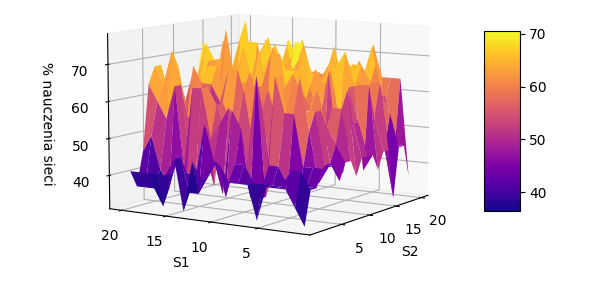
\includegraphics[width=12cm]{s1000epok1.png}
\caption{Wykres wypływu S1, S2 na poprawność klasyfikacji (maks. 1000 epok)}
\end{figure}

\begin{figure}[H]
\label{s1000epok2}
\centering
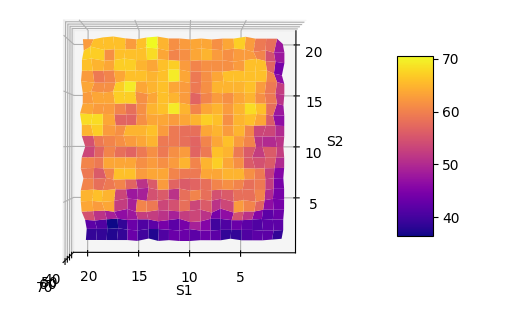
\includegraphics[width=12cm]{s1000epok2.png}
\caption{Wykres wypływu S1, S2 na poprawność klasyfikacji (maks. 1000 epok)}
\end{figure}

W wyniku tego eksperymentu okazało się, że dla tych parametrów sieć nie przekracza skuteczności równej $77,27\%$. Skuteczność tę osiąga dla 19 neuronów na warstwie I i 19 neuronów na warstwie II oraz dla 16 neuronów na warstwie I i 11 neuronów na warstwie II.

\subsubsection{Badania dla 2000 epok}
Ze względu na niezadowalające wyniki eksperymentu dla maksmalnej liczby epok równej 1000, liczba ta została zwiększona dwukrotnie. Dalsze eksperymenty przeprowadzono więc dla 2000 epok. Pozostałe parametry pozostały bez zmian.

\begin{figure}[H]
\label{s2000epok1}
\centering
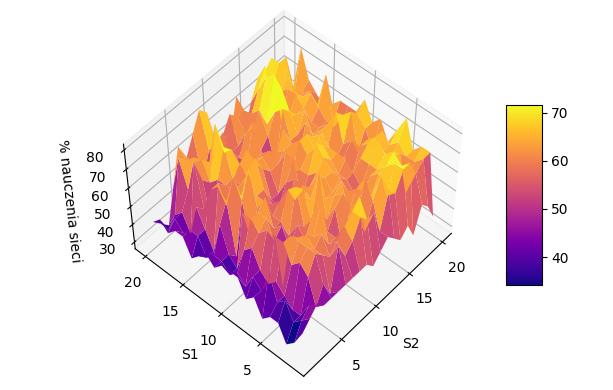
\includegraphics[width=12cm]{s2000epok1.png}
\caption{Wykres wypływu S1, S2 na poprawność klasyfikacji (maks. 2000 epok)}
\end{figure}

\begin{figure}[H]
\label{s2000epok2}
\centering
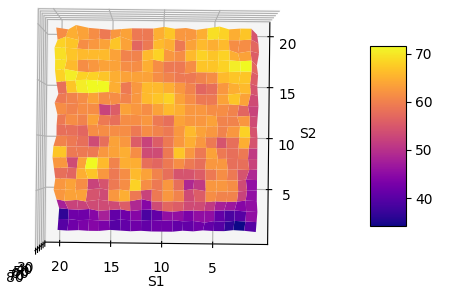
\includegraphics[width=10cm]{s2000epok2.png}
\caption{Wykres wypływu S1, S2 na poprawność klasyfikacji (maks. 2000 epok)}
\end{figure}

Sieć osiąga najlepszą skuteczność równą $81,82\%$ dla 17 neuronów na warstwie I i 7 neuronów na warstwie II oraz dla 17 neuronów na warstwie I i 15 neuronów na warstwie II. Został także przeprowadzony eksperyment dla maks. liczby epok równej 5000, jednak nie zmieniło to w żadnym stopniu skuteczności sieci.

\subsection{Eksperyment 2 - badanie parametrów $lr_{inc}$ oraz $lr_{dec}$}
Na potrzeby eksperytmentu 2 przyjęto parametry uczenia określone w tabeli \ref{tab2}, zmianie poddane zostały parametry:
\begin{itemize}
\item learning rate accelerate - w przedziale $< 0.9; 1.9 >$, ze skokiem co 0.05
\item learning rate decelerate - w przedziale $< 0.1; 1.1 >$, ze skokiem co 0.05
\end{itemize}


\begin{lstlisting}[language=Python,caption=Algorytm realizujący eksperyment 2,label={eks2}]
import sys
import network
from data import loadData
import pandas as pd
import numpy as np
from tabulate import tabulate
trainData, testData = loadData()
lr_inc_vec=np.arange(0.9,1.91,0.05)
lr_dec_vec=np.arange(0.1,1.11,0.05)
results = []
name=sys.argv[3]
name='result'+name+'.csv'
for lr_inc in lr_inc_vec:
    for lr_dec in lr_dec_vec:
        result = [lr_inc,lr_dec]
        net = network.Network([9, int(sys.argv[1]), int(sys.argv[2]), 6])
        result.extend(net.SGD(trainData,2000,len(trainData),0.1,testData,0.25,lr_inc,lr_dec))
        results.append(result)

results=pd.DataFrame(results)
results.to_csv(name,index=None,header=None)

\end{lstlisting}

\newpage

\subsubsection{Badania dla $S1=17$, $S2=7$}

\begin{figure}[H]
\centering
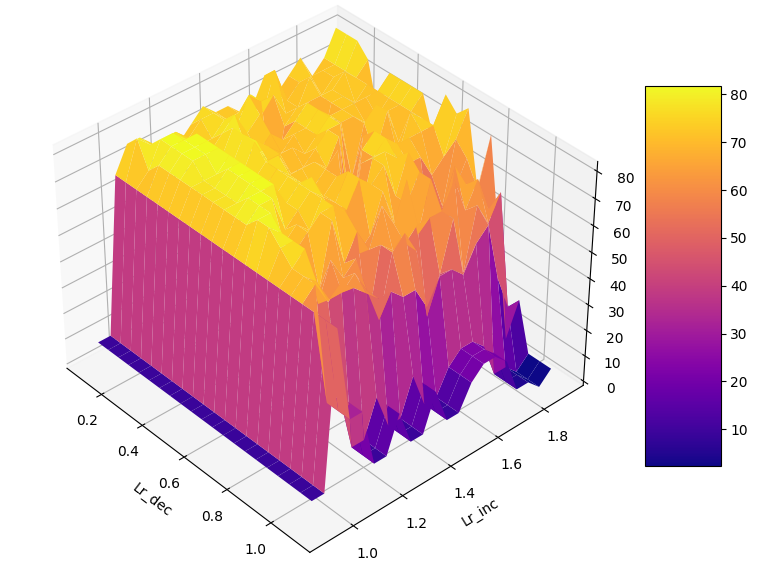
\includegraphics[width=12cm]{eks2-17-7-1.png}
\caption{Zależność poprawności klasyfikacji od $lr_{inc}$ oraz $lr_{dec}$ dla $S1=17$, $S2=7$}
\label{eks2-17-7-1}
\end{figure}

\begin{figure}[H]
\centering
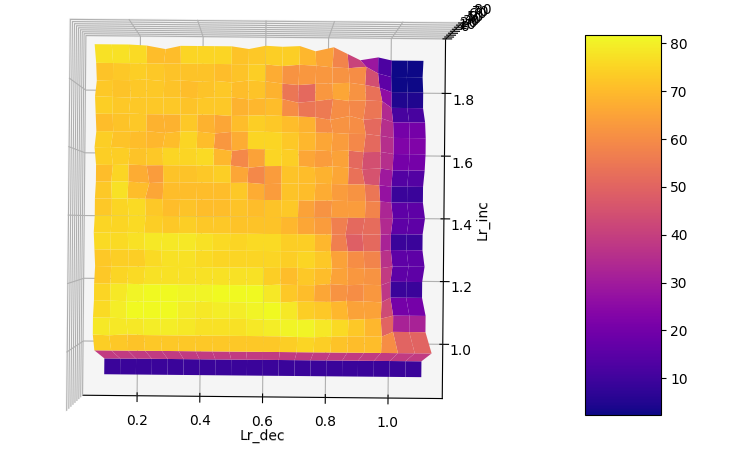
\includegraphics[width=12cm]{eks2-17-7-2.png}
\caption{Zależność poprawności klasyfikacji od $lr_{inc}$ oraz $lr_{dec}$ dla $S1=17$, $S2=7$}
\label{eks2-17-7-2}
\end{figure}

Rysunki \ref{eks2-17-7-1}, oraz \ref{eks2-17-7-2}, przedstawiają powierzchnię funkcji procentowej wartości poprawności klasyfikacji w zależności od
wartości parametru learning rate accelerate oraz learning rate decelerate. Dla S1= 17, S2 = 7 największą poprawność uczenia osiągnięto dla wartości z przedziału $lr_{inc}  = [1.0; 1.1]$, oraz $lr_{dec} = [0.2; 0.6]$ - $81,81\%$. Natomiast najgorszy wynik uzyskano gdy $lr_{inc}$ wynosił 0.9 lub $lr_{dec}$ był większy niż 1.

\subsubsection{Badania dla $S1=17$, $S2=15$}

\begin{figure}[H]
\centering
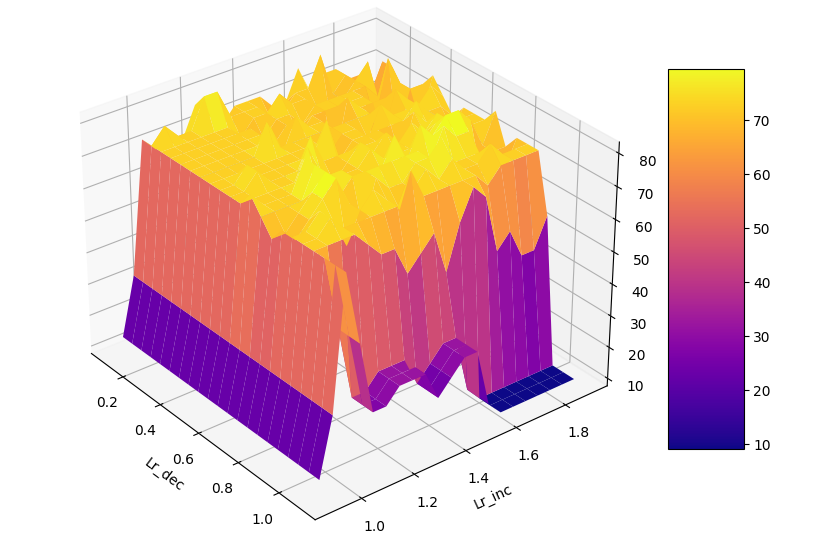
\includegraphics[width=12cm]{eks2-17-15-1.png}
\caption{Zależność poprawności klasyfikacji od $lr_{inc}$ oraz $lr_{dec}$ dla $S1=17$, $S2=15$}
\label{eks2-17-15-1}
\end{figure}

\begin{figure}[H]
\centering
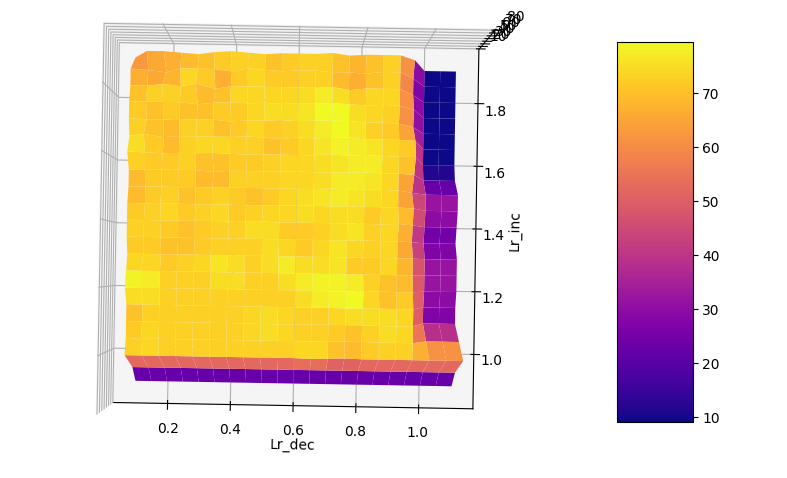
\includegraphics[width=12cm]{eks2-17-15-2.png}
\caption{Zależność poprawności klasyfikacji od $lr_{inc}$ oraz $lr_{dec}$ dla S1=17, S2=15}
\label{eks2-17-15-2}
\end{figure}

Na rysunkach \ref{eks2-17-15-1}, oraz \ref{eks2-17-15-2} można zauważyć, że dla S1= 17, S2 = 15 największą poprawność uczenia osiągnięto dla wartości $lr_{inc}  = [1.20; 1.25]$, $lr_{dec} = [0.65; 0.8]$ oraz $lr_{inc}  = 1.4$, $lr_{dec} = 0.9$. Natomiast najgorsze wyniki uzyskano gdy $lr_{inc}$ wynosił 0.9 lub $lr_{dec}$ był większy niż 1.

Porównując przedstawione wyżej wykresy i wartości, można wywnioskować, że sieć w parametrach S1= 17, S2 = 7 jest lepiej uwarunkowana dla badanego zestawu danych. 


\subsection{Eksperyment 3 - badanie parametru er}
W kolejnym z eksperymentów zbadano wpływ parametru $er$ na procentową wartość nauczenia sieci. Domyślnie parametr ten wynosił $1.04$. Na potrzeby eksperymentu zmieniano wartość $er$ w zakresie $[1.01; 1.07]$. Badania przeprowadzono dla maksymalnej liczby 2000 epok,  $lr_{inc}  = 1.05$, $lr_{dec} = 0.7$ oraz parametrów S1 = 17, S2 = 7. Listing \ref{eks3} przedstawia kod, którego użyto do eksperymentu.

\begin{lstlisting}[language=Python,caption=Algorytm realizujący eksperyment 3,label={eks3}]
import network
from data import loadData
import pandas as pd
import numpy as np
from tabulate import tabulate
trainData, testData = loadData()
er_ratio_vec=np.arange(1.01,1.071,0.01)
results = []
for er in er_ratio_vec:
    result = [er]
    net = network.Network([9, 17, 7,  6],err=er)
    print('Er: {0}'.format(er))
    result.extend(net.SGD(trainData,2000,len(trainData),0.1,testData,0.25,1.05,0.7))
    results.append(result)

results=pd.DataFrame(results)
results.to_csv('new_resulty_1.csv',index=None,header=None)

\end{lstlisting}

\begin{figure}[H]
\centering
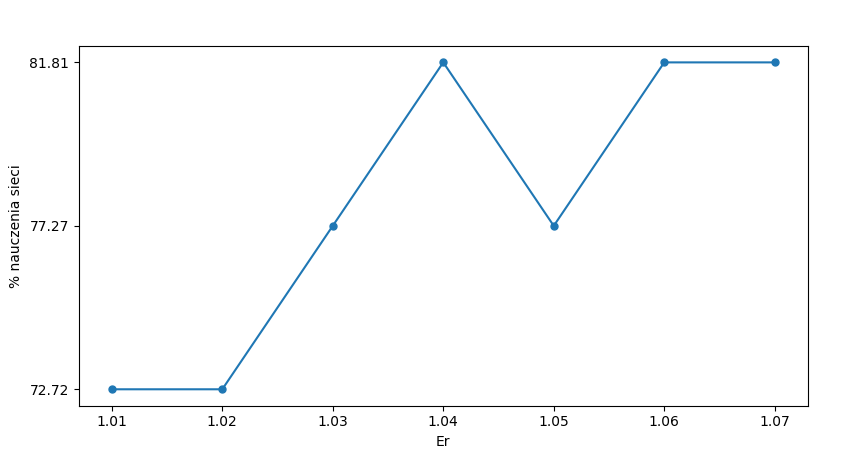
\includegraphics[width=12cm]{eks3.png}
\caption{Wykres wpływu parametru er na poprawność klasyfikacji}
\label{ryseks3}
\end{figure}

Rysunek \ref{ryseks3} obrazuje wyniki wykonanego badania. Warstość domyślna parametru $er = 1.04$ jest dobrze dobrana, ponieważ daje najwyższy wynik nauczenia sieci. 

\clearpage
\section{Podsumowanie i wnioski końcowe}

Cel projektu, tj. zrealizowanie sztucznej sieci neuronowej uczonej algorytmem wstecznej propagacji błędu z przyśpieszeniem metodą adaptacyjnego współczynnika uczenia (trainbpa) uczącej się diagnozowania choroby został zrealizowany. W tym celu wykorzystano własną implementację sieci neuronowej napisanej w jęyku Python na podstawie książki Michaela Nielsena \cite{nielsen}. 

Zadany zbiór okazał się być zbiorem trudnym do nauczenia. Procentowa dokładność klasyfikacji nie przekraczała nigdy $81,82\%$. 

Eksperymenty pozwoliły na określenie optymalnych wartości parametrów, dla których sieć osiąga najlepsze wyniki. 

Pierwszy eksperyment polegał na dostosowaniu ilości neuronów w warstwie I i II. Wyniki eksperymentu nie były zadowalające, najlepszy wynik osiągnięty przez sieć wynosił $81,82\%$ i został uzyskany dla maksymanej liczby epok równej 2000 oraz parametrów $S1=17$, $S2=7$ i $S1=17$, $S2=15$. 

Celem drugiego eksperymentu było wyznaczenie optymalnych wartości parametrów $lr_{inc}$ oraz $lr_{dec}$. Badanie to przeprowadzono dla najlepszych wyników otrzymanych z eksperymentu 1. Okazało się, iż istnieje wiele wartości badanych parametrów, dla których sieć uczy się dobrze. Na podstawie uzyskanych wykresów można także wywnioskować, że sieć jest lepiej uwarunkowana dla $S1 = 17$ oraz $S2 = 7$.

Trzeci, ostatni eksperyment przeprowadzono w celu wyznaczenia najbardziej optymalnego parametru $er$. Obserwując wynik badania, można zauważyć, że sieć osiąga najlepsze wartości dla $er = \{1.04, 1.06, 1.07\}$. 

Przeprowadzone eksperymenty pozwoliły na ustalenie optymalnych wartości parametrów, dla których sieć osiągała najlepszy wynik poprawności klasyfikacji. Badania te wykazały, że domyślne parametry z programu Matlab są najkorzystniejsze. 

\clearpage


\addcontentsline{toc}{section}{Literatura}

\begin{thebibliography}{4}
\bibitem{dane} UCI Machine Learning Repository\\https://archive.ics.uci.edu/ml/datasets/Wine [Dostęp 14.05.2022 r.]
\bibitem{nielsen} Michael A. Nielsen, "Neural Networks and Deep Learning", Determination Press, 2015
\bibitem{norm} http://sztuczna-inteligencja.eprace.edu.pl/1001,Funkcje-normalizacji.html [Dostęp 14.05.2022 r.]
\bibitem{zajdel2}dr hab. inż. Roman Zajdel prof. PRz, PRz, KIiA, Sztuczna inteligencja, Laboratorium, Ćw8 Sieć jednokierunkowa jednowarstwowa\\
http://materialy.prz-rzeszow.pl/pracownik/pliki/34/sztuczna-inteligencja-cw8-siec-jednowarstw.pdf [Dostęp 09.06.2022 r.]
\bibitem{zajdel1}dr hab. inż. Roman Zajdel prof. PRz, PRz, KIiA, Sztuczna inteligencja, Laboratorium, Ćw9 Sieć jednokierunkowa wielowarstwowa\\
http://materialy.prz-rzeszow.pl/pracownik/pliki/34/sztuczna-inteligencja-cw9-siec-wielowarstw.pdf [Dostęp 09.06.2022 r.]
\bibitem{mamczur}https://miroslawmamczur.pl/czym-jest-i-jak-sie-uczy-sztuczna-siec-neuronowa/ [Dostęp 21.05.2022 r.]
\bibitem{leksykon} R. Tadeusiewicz, M. Szaleniec „Leksykon sieci neuronowych”, Wrocław 2015


\end{thebibliography}

\clearpage


\end{document} 
